% Experimental Workflow / Baseline Comparison Figure (standalone TikZ)
% Compile with: pdflatex baselines.tex
\documentclass[border=5pt]{standalone}
\usepackage{tikz}
\usetikzlibrary{shapes.geometric, arrows.meta, positioning, fit, calc}

\begin{document}
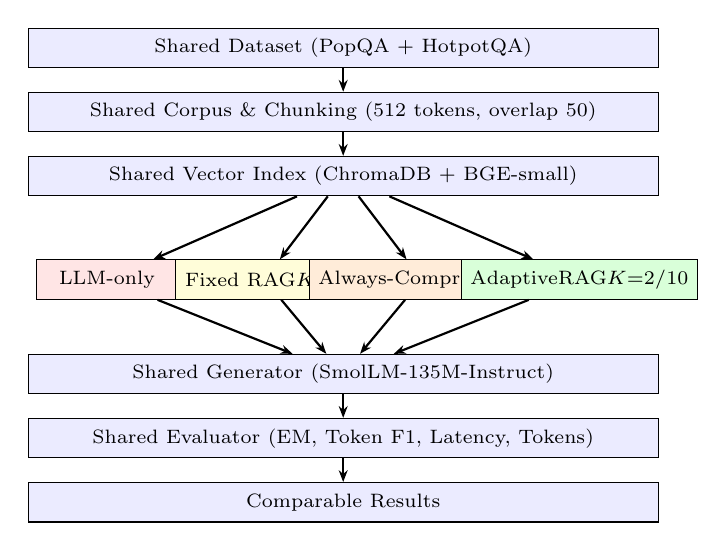
\begin{tikzpicture}[
    node distance=0.5cm and 0.6cm,
    block/.style={rectangle, draw, text centered, minimum width=1.8cm, minimum height=0.5cm, font=\scriptsize},
    shared/.style={rectangle, draw, text centered, minimum width=8cm, minimum height=0.5cm, font=\scriptsize, fill=blue!8},
    arrow/.style={-{Stealth[length=1.5mm]}, thick},
]

% Shared top
\node[shared] (dataset) {Shared Dataset (PopQA + HotpotQA)};
\node[shared, below=0.3cm of dataset] (corpus) {Shared Corpus \& Chunking (512 tokens, overlap 50)};
\node[shared, below=0.3cm of corpus] (index) {Shared Vector Index (ChromaDB + BGE-small)};

% Four baselines
\node[block, below=0.8cm of index, xshift=-3.0cm, fill=red!10] (a) {LLM-only};
\node[block, below=0.8cm of index, xshift=-1.0cm, fill=yellow!15] (b) {Fixed RAG\\$K{=}5$};
\node[block, below=0.8cm of index, xshift=1.0cm, fill=orange!15] (c) {Always-Compr.\\$K{=}10$};
\node[block, below=0.8cm of index, xshift=3.0cm, fill=green!15] (d) {AdaptiveRAG\\$K{=}2/10$};

% Shared bottom
\node[shared, below=0.8cm of index, yshift=-1.2cm] (gen) {Shared Generator (SmolLM-135M-Instruct)};
\node[shared, below=0.3cm of gen] (eval) {Shared Evaluator (EM, Token F1, Latency, Tokens)};
\node[shared, below=0.3cm of eval] (results) {Comparable Results};

% Arrows
\draw[arrow] (dataset) -- (corpus);
\draw[arrow] (corpus) -- (index);

\draw[arrow] (index) -- (a);
\draw[arrow] (index) -- (b);
\draw[arrow] (index) -- (c);
\draw[arrow] (index) -- (d);

\draw[arrow] (a) -- (gen);
\draw[arrow] (b) -- (gen);
\draw[arrow] (c) -- (gen);
\draw[arrow] (d) -- (gen);

\draw[arrow] (gen) -- (eval);
\draw[arrow] (eval) -- (results);

\end{tikzpicture}
\end{document}
